\documentclass[chapterprefix=off]{rtxreport}

\usepackage{pdflscape}

\author{Louis Opter}
\title{Cahier des charges pour 2012}

\rtxdoctype{Test Document}
\rtxdocstatus{Brouillon}
\rtxdocversion{0.3}

\rtxdochistory
{
0.1 & 11/03/2011 & Louis Opter & Reprise du CDC1 \\
\hline
0.2 & 17/03/2011 & Louis Opter & Prise en compte des remarques faites lors du DA2 \\
\hline
0.3 & 19/03/2011 & Louis Opter & Ajout du schéma du compilateur \\
}

\begin{document}

\maketitle

\begin{abstract}
\rtx\ est un générateur, multi-plateformes, de pilotes de périphériques
matériels. Le fonctionnement du périphérique est décrit dans le langage
spécialisé \rtx\ avant d'être compilé vers un module noyau écrit en C pour
Linux, Windows ou OpenBSD.
\end{abstract}

\rtxmaketitleblock

\tableofcontents

\chapter{Introduction}

\section{\rtx}

% Rajouter un logo avec wrapfig

Ce document est le cahier des charges pour le projet \rtx\  2012. Il comporte
une description du travail à accomplir pour achever ce projet. \rtx\  est un
générateur de pilote de périphériques d'ordinateurs multi-plateformes.

\rtx\ est réalisé par l'équipe EIP \rtx\ 2012 et s'inscrit dans la continuité
du travail effectué par l'équipe 2009.

Ce document s'adresse aux développeurs \rtx\  et à l'équipe du laboratoire EIP.
Il décrit le projet \rtx, ses buts, ses moyens et ses limites.

Ce projet est réalisé en partenariat avec le LSE : \emph{«~Laboratoire Système et
Sécurité Epita et Epitech~»}.

\section{Laboratoire EIP}

% Rajouter un logo eip avec wrapfig

EIP est un acronyme pour : \emph{«~Epitech Innovative Project~»}.

Les EIP désignent les projets de fin d'études réalisés par les étudiants
d'Epitech à partir de leur troisième année.

L'équipe pédagogique du laboratoire EIP prend en charge les étudiants sur toute
la durée de leurs EIP avec des suivis, des corrections et une infrastructure.

\chapter{\rtx\ 2009}

\section{Problématique}

Écrire un pilote matériel requiert des connaissances approfondies sur comment le
matériel et le système fonctionnent. Les pilotes sont lancés avec un haut niveau
de privilège et peuvent causer des désastres si quelque chose est mal fait
(tel qu'un arrêt brutal de la machine).

Chaque plateforme propose ses propres interfaces de communication et les
pilotes doivent être écrits pour chacune d'elles.

Au final, il semble évident que des logiciels sont manquants pour contrer ces
problèmes :
\begin{itemize}
\item Séparation entre les compétences matériel et logicielle ;
\item Temps de développement ;
\item Réutilisation du code.
\end{itemize}

\section{Vue d'ensemble du projet}

Le projet \rtx\ 2009 était divisé en trois parties :
\begin{enumerate}
\item Le DSL\footnote{\emph{Domain Specific Language}} qui décrit un pilote
périphérique ;
\item La \BL\ est une bibliothèque de patrons utilisée lors de la génération
du pilote ;
\item Un compilateur qui traduit le DSL \rtx\ et génère un pilote.
\end{enumerate}

Le projet comporte aussi une documentation abondante sur le DSL, la \BL\ et une
référence, \emph{«~l'état de l'art~»} sur la rédaction de pilotes de
périphériques. Cette documentation s'adresse aux développeurs \rtx\ (aussi bien
du groupe d'EIP ou des contributeurs externes) et aux utilisateurs.

Actuellement, \rtx\ est une preuve de concept qui peut générer un pilote RS-232.

\chapter{Objectifs pour 2012}

L'EIP \rtx\ 2012 a quatre objectifs :
\begin{enumerate}
\item Rendre le développement publique sous des licences Open Source ;
\item Contribuer à l'état de l'art qui ne couvre que les modules noyaux
(\emph{LKM}) et un pilote série RS-232 ;
\item Dégager de nouveaux concepts clefs de l'état de l'art sur
des bus utilisés couramment tel que PCI ou I\textsuperscript{2}C et leurs
mécanismes associés (interruptions, asynchrone, DMA) ;
\item Devenir plus actif dans la communauté Open Source.
\end{enumerate}

Au delà de l'EIP, l'équipe \rtx\ souhaite rendre le projet attractif pour la
communauté de développeurs de pilotes open source.

\chapter{Contraintes}

\rtx\ 2012 conserve la même organisation qu'en 2009 (DSL, compilateur et \BL).

\section{Le DSL}

Le DSL \rtx\ doit :
\begin{itemize}
\item Décrire simplement et efficacement un pilote périphérique ;
\item Être capable d'intégrer des morceaux de code C ;
\item Être naturel au possible pour un programmeur et un ingénieur en
électronique ;
\item Avoir une syntaxe robuste et et une forte sémantique.
\end{itemize}

Le code C généré doit être robuste puisque le système d'exploitation dépend de lui.

L'organisation du DSL change par rapport à la version 2009 : au front-end et au
back-end du langage s'ajoute le middle-end qui va être capable de relier les
deux parties en déclarant les types, séquences (algorithmes) et variables
disponibles.

\section{Le compilateur}

Avec le multi-plateforme, la capacité de réutiliser le code devient un enjeu.
Pour chaque plateforme, le générateur de pilote doit :
\begin{itemize}
\item Être installable sur chaque système supporté ;
\item Être capable d'être lancé en ligne de commande ;
\item Vérifier la syntaxe du DSL ;
\item Vérifier la sémantique de ses entrées ;
\item Utiliser CodeWorker\cite{CodeWorker} ;
\item Utiliser les outils natifs à chaque plateforme.
\end{itemize}

L'architecture du compilateur va être revue pour prendre en compte les
changements sur le DSL, voir figure \ref{diagramme} page \pageref{diagramme}.

\begin{figure}
\begin{center}
\caption{Architecture du compilateur}
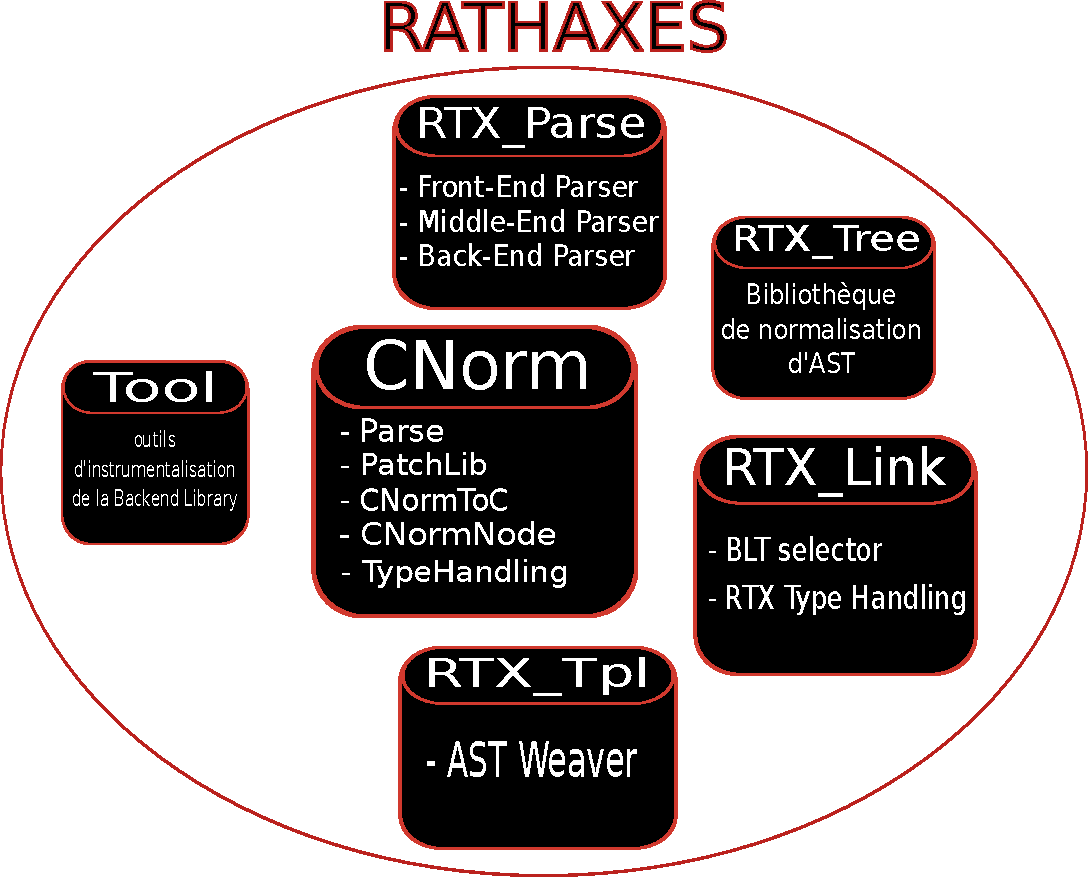
\includegraphics[width=0.95\textwidth]{../../../../doc/rathaxes/technical/diagramme_architecture.pdf}
\label{diagramme}
\end{center}
\end{figure}

\section{La \BL}

La \BL\ doit :
\begin{itemize}
\item Contenir le code des patrons utilisés par le compilateur ;
\item Être amélioré avec la gestion des bus ;
\item Mise \`a jour avec la nouvelle version du compilateur.
\end{itemize}

\section{Support de l'asynchrone}

Actuellement, \rtx\ supporte seulement la communication synchrone avec les
périphériques. Cependant, la plupart des périphériques communiquent de manière
asynchrone (avec des mécanismes d'interruptions) et sa gestion dans le DSL est
incontournable.

\section{Licence}

En tant que projet scientifique \rtx\ est distribué selon deux licences open
source :
\begin{description}
\item[GPLv3 :] Pour le compilateur, afin de garder une propriété intellectuelle
et de s'assurer qu'il n'existera qu'une seule version du langage ;
\item[BSD :] Pour la \BL\ afin de rendre possible l'adoption de \rtx\ par des
entreprises.
\end{description}

\chapter{Contrôle du projet}

\section{Statut de l'association}

\rtx\ est une association loi de 1901. Une mise à jour des statuts est
prévue pour fin 2010.

Un compte en banque géré par l'association sera créé afin de subvenir aux
besoins du projet.

Dépenses prévues :
\begin{itemize}
\item Voyage (RMLL Strasbourg\footnote{Rencontres Mondiales du Logiciel
Libre (\url{http://rmll.info/}).}, T-Dose
Eindhoven\footnote{\url{http://www.t-dose.org/}.}) ;
\item Nom de domaine (rathaxes.org).
\end{itemize}

En tant qu'association, \rtx\ peut recevoir des donations.

\section{Environnement de travail}

\begin{itemize}
\item Le LSE est capable de subvenir à la plupart des besoins en matériel ;
\item Trois systèmes d'exploitation seront utilisés pour les recherches et les
tests, trois machines x86 seront donc nécessaires. Cependant elles pourront
être virtualisées afin d'unifier l'environnement de test ;
\item Les périphériques de test seront obtenus à partir du LSE ou achetés si
besoin ;
\item Le code est hébergé sur GoogleCode : \url{http://code.google.com/p/rathaxes/} ;
\item Le wiki du google code propose un point de départ pour installer et
tester \rtx\ ;
\item Le code est versionné avec
Mercurial\footnote{\url{http://mercurial.selenic.com/}.} ;
\item Le gestionnaire de bogues (tickets) est public et utilisé pour développer
le projet ;
\item Le code, les tickets ainsi que la documentation doivent être écrits en
anglais ;
\item En plus des courriels Epitech, chaque membre du projet doit être présent
sur le canal IRC suivant: \url{irc://rathaxes@irc.freenode.org}.
\end{itemize}

\section{Planification}

\rtx\ 2012 est la somme de plusieurs étapes :

\begin{enumerate}
\item Étudier des pilotes existant sur chaque plateforme ;
\item Écrire des pilotes sur chaque plateforme ;
\item Définir les concepts à implémenter dans le DSL ;
\item Commencer à travailler avec le code de \rtx\ ;
\item Mettre à jour le DSL ;
\item Écrire des pilotes avec \rtx\ ;
\item Participer aux RMLL à Strasbourg et au T-Dose à Eindhoven.
\end{enumerate}

\begin{landscape}
\begin{table}
\centering
\captionabove{Diagramme de Gantt pour 2011}
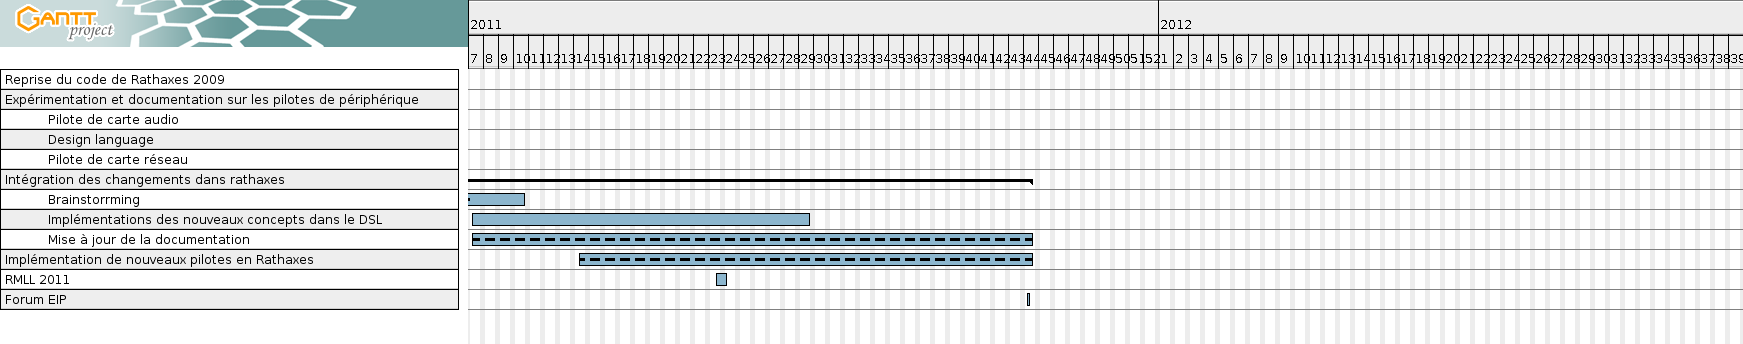
\includegraphics[scale=0.55]{../../gantt/ganttRathaxes_v2}
\end{table}
\end{landscape}

\rtxbibliography

\end{document}
